%!TEX root =../../../course-notes.tex
% ^ leave for LaTeXTools build functionality

\begin{applicationActivities}



\begin{activity}{5}
  How many vectors are required to span \(\IR^2\)?
  Sketch a drawing in the \(xy\) plane to support your answer.
  \begin{enumerate}[(a)]
  \item $1$
  \item $2$
  \item $3$
  \item $4$
  \item Infinitely Many
  \end{enumerate}
\end{activity}

\begin{activity}{5}
  How many vectors are required to span \(\IR^3\)?
  \begin{enumerate}[(a)]
  \item $1$
  \item $2$
  \item $3$
  \item $4$
  \item Infinitely Many
  \end{enumerate}
\end{activity}

\begin{fact}
  At least \(n\) vectors are required to span \(\IR^n\).

  \begin{center}
  \begin{tikzpicture}[scale=0.5]
    \draw[<->] (-4,0) -- (4,0);
    \draw[<->] (0,-4) -- (0,4);
    \draw[blue!50] (2,-4) -- (-2,4);
    \draw[thick,blue,->] (0,0) -- (1,-2);
  \end{tikzpicture}
  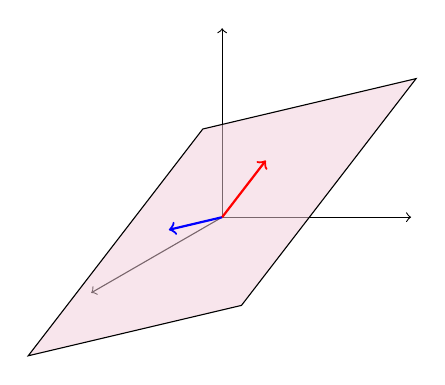
\begin{tikzpicture}[x={(210:0.8cm)}, y={(0:1cm)}, z={(90:1cm)},scale=0.4]
    \draw[->] (0,0,0) -- (6,0,0);
    \draw[->] (0,0,0) -- (0,6,0);
    \draw[->] (0,0,0) -- (0,0,6);
    \draw[fill=purple!20,fill opacity=0.5]
      (-2,-2,2) -- (6,-2,-2) -- (2,2,-2) -- (-6,2,2) -- (-2,-2,2);
    \draw[thick,blue,->] (0,0,0) -- (1,-1,0);
    \draw[thick,red,->] (0,0,0) -- (-2,0,1);
  \end{tikzpicture}
  \end{center}
\end{fact}

\begin{activity}{15}
  Choose a vector \(\begin{bmatrix}\unknown\\\unknown\\\unknown\end{bmatrix}\)
  in \(\IR^3\) that is not in
  \(\vspan\left\{\begin{bmatrix}1\\-1\\0\end{bmatrix},
  \begin{bmatrix}-2\\0\\1\end{bmatrix}\right\}\) by using CoCalc to verify that
  \(
    \RREF
    \begin{bmatrix}[cc|c]1&-2&\unknown\\-1&0&\unknown\\0&1&\unknown\end{bmatrix}
      =
    \begin{bmatrix}[cc|c]1&0&0\\0&1&0\\0&0&1\end{bmatrix}
  \).
  (Why does this work?)
\end{activity}

\begin{fact}
  The set \(\{\vect v_1,\dots,\vect v_m\}\) fails to span all of \(\IR^n\)
  exactly when \(\RREF[\vect v_1\,\dots\,\vect v_m]\) has a row of zeros:
  \[\begin{bmatrix}[cc]1&-2\\-1&0\\0&1\end{bmatrix}\sim
  \begin{bmatrix}[cc]1&0\\0&1\\0&0\end{bmatrix}\Rightarrow
  \begin{bmatrix}[cc|c]1&-2&a\\-1&0&b\\0&1&c\end{bmatrix}\sim
  \begin{bmatrix}[cc|c]1&0&0\\0&1&0\\0&0&1\end{bmatrix}
  \text{for some choice of vector} \begin{bmatrix} a \\ b \\ c \end{bmatrix} \]
\end{fact}

\begin{activity}{5}
  Consider the set of vectors \(S=\left\{
  \begin{bmatrix}2\\3\\0\\-1\end{bmatrix},
  \begin{bmatrix}1\\-4\\3\\0\end{bmatrix},
  \begin{bmatrix}2\\0\\0\\3\end{bmatrix},
  \begin{bmatrix}0\\3\\5\\7\end{bmatrix},
  \begin{bmatrix}3\\13\\7\\16\end{bmatrix}
  \right\}
  \).
  Does
  \(\IR^4=\vspan S\)?
  % \begin{subactivity}
  % Find a linear combination of vectors in \(S\) that equals
  % \(\begin{bmatrix}-1\\10\\7\\14\end{bmatrix}\).
  % \end{subactivity}
\end{activity}

\begin{activity}{10}
  Consider the set of third-degree polynomials 
  \begin{align*}
  S=\{
  &2x^3+3x^2-1,
  2x^3+3,
  3x^3+13x^2+7x+16, \\
  &-x^3+10x^2+7x+14,
  4x^3+3x^2+2 \} .
  \end{align*}
  Does
  \(\P^3=\vspan S\)?
  (Hint: first rewrite the question so it is about Euclidean vectors.)
  % \begin{subactivity}
  % Find a vector in \(\IR^4\) that is not in \(\vspan S\).
  % \end{subactivity}
\end{activity}

\begin{activity}{5}
Consider the set of matrices
\[ S = \left\{
		\begin{bmatrix} 1 & 3 \\ 0 & 1 \end{bmatrix},
		\begin{bmatrix} 1 & -1 \\ 1 & 0 \end{bmatrix},
		\begin{bmatrix} 1 & 0 \\ 0 & 2 \end{bmatrix}
		\right\} \]
Does \(M_{2,2} = \vspan S\)?
\end{activity}

\begin{activity}{5}
Let \(\vec{v}_1, \vec{v}_2, \vec{v}_3 \in \IR^7\) be three vectors, and suppose \(\vec{w}\) is another vector with \(\vec{w} \in \vspan \left\{ \vec{v}_1, \vec{v}_2, \vec{v}_3 \right\}\).  What can you conclude about \( \vspan \left\{ \vec{w}, \vec{v}_1, \vec{v}_2, \vec{v}_3 \right\} \) ?
\begin{enumerate}[(a)]
\item \( \vspan \left\{ \vec{w}, \vec{v}_1, \vec{v}_2, \vec{v}_3 \right\} \) is larger than \( \vspan \left\{ \vec{v}_1, \vec{v}_2, \vec{v}_3 \right\} \).
\item \( \vspan \left\{ \vec{w}, \vec{v}_1, \vec{v}_2, \vec{v}_3 \right\}  = \vspan \left\{ \vec{v}_1, \vec{v}_2, \vec{v}_3 \right\} \).
\item \( \vspan \left\{ \vec{w}, \vec{v}_1, \vec{v}_2, \vec{v}_3 \right\} \) is smaller than \( \vspan \left\{ \vec{v}_1, \vec{v}_2, \vec{v}_3 \right\} \).
\end{enumerate}
\end{activity}

\end{applicationActivities}
